\chapter{Detección de vulnerabilidades en imaxes}
\minitoc
\clearpage

\section{Introdución}

Cando traballamos cun entorno baseado en contedores, debemos ter presente que, xunto con todas as vantaxes que estes aportan, como pode ser o despregamento de entornos áxiles, tamén estamos a introducir novos elementos no noso sistema que poden chegar a supor novos posíbeis vectores de ataque. A implicación de novos sistemas operativos e librarías no conxunto do novo sistema poden levar a aparición de novas vulnerabilidades que non poden ser tan doadamente controladas coma se estivésemos a tratar co noso sistema principal (a máquina anfitrioa). Este feito vén, precisamente, asociado á simplicidade de despregamento destes entornos.\\

Cabe a posibilidade de que un usuario, de xeito intencionado ou non, despregue un contedor con vulnerabilidades incluídas no seu interior e así supor unha punto de entrada para a posterior execución de \textit{malware}. Este feito vese agravado se temos en conta que o que se desexa facer é acadar un sistema multiusuario onde cada quen poida despregar os seus propios contedores. Para minimizar as posibilidades de que este fenómeno aconteza, é boa idea descargar e empregar soamente contedores obtidos de fontes fiábeis, das cales coñezamos o seu lexítimo creador.

\section{Portais de almacenamento de contedores}

Así, entran en xogo numerosos portais de almacenamento de contedores, como poden ser Docker Hub\footnote{\url{https://hub.docker.com/}} ou Singularity Hub\footnote{\url{https://singularity-hub.org/}}. Ditos portais poden amosarnos información útil para comprender as implicacións de seguridade que pode ter a emprega das imaxes dos contedores aí almacenados. Por exemplo, en primeiro lugar identificarase o autor de dito contido, dándonos a coñecer se se trata de material oficial, ou provinte ou non dunha fonte da nosa confianza. Ademais, os portais poden contar con medidas máis avanzadas no referente á seguridade, que permitan un maior coñecemento do que estamos a descargar. Para aclarar a hipótese exposta, mostrarase un exemplo sobre unha das plataformas previamente nomeadas.\\

Mais antes de comezar con dito exemplo, cómpre ter un par de termos claros: un contedor é lanzado cando corremos unha imaxe. Polo tanto, unha imaxe constitúe un paquete executábel que inclúe todo o necesario para correr unha aplicación (código, librarías, variábeis de entorno, ficheiros de configuración...). Pola contra, un contedor é a instancia en tempo de execución dunha imaxe, é dicir, no que a imaxe se transforma na memoria cando é executada. \cite{docker-get-started}\\

\subsection[Exemplo práctico: Docker Hub]{Exemplo práctico: estudo das medidas avanzadas de seguridade nunha plataforma de almacenamento: Docker Hub}

\subsubsection{Introdución}

O Docker Hub trátase dun servizo baseado na nube para o rexistro de contedores, así como permitir construír imaxes e probalas. Tamén constitúe un recurso centralizado para o descubrimento, distribución, xestión de cambios e automatización do fluxo de traballo en toda a liña de desenvolvemento. \cite{dockerHubExp}\\

Este servizo permítenos procurar entre multitude de imaxes, a través das cales podemos obter sistemas completamente configurados para o seu despregamento e posta en marcha. Outra característica a ter en conta é que as novas imaxes non teñen por que ser refeitas de cero, senón que é posíbel estender imaxes xa existentes, habendo así unha relación pai-fillo entre imaxes e podendo facer ramas doutros repositorios. Concretando un pouco máis, cada imaxe de Docker está composta por unha lista de capas de só lectura. Na máquina anfitrioa, cada capa será almacenada coma un ficheiro \textit{tar} cun único directorio. As capas son empilladas xerarquicamente, onde o seu orde queda especificado nun ficheiro \gls{JSON} de configuración  \cite{studySecurityDockerHub}. Polo tanto, parte destas capas poden ser reempregadas integramente cando creamos unha nova imaxe en base a outra xa existente.

\subsubsection{Fontes}

Cando descargamos estes contedores debemos prestar especial atención á súa orixe. Deste xeito, a plataforma permítenos distinguir entre contedores oficiais, que son aqueles provintes dos propios desenvolvedores dunha tecnoloxía; e entre repositorios públicos dun determinado autor. Os repositorios oficiais son considerados de maior confianza, posto que son dados polos propios creadores da tecnoloxía, e son sometidos a probas de seguridade por parte do Docker Hub, namentres que os repositorios públicos doutros usuarios simplemente poden ser descargados, pero as súas medidas previas de seguridade son moito máis limitadas.\\

\begin{figure}
\centerline{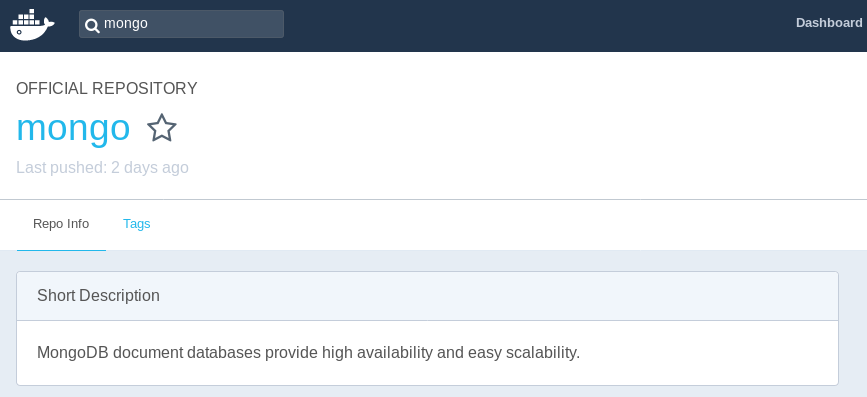
\includegraphics[width=15cm]{figuras/dockerOficial}}
\caption{Exemplo dun repositorio oficial no Docker Hub.}
\label{dockerOficial}
\end{figure}

\begin{figure}
\centerline{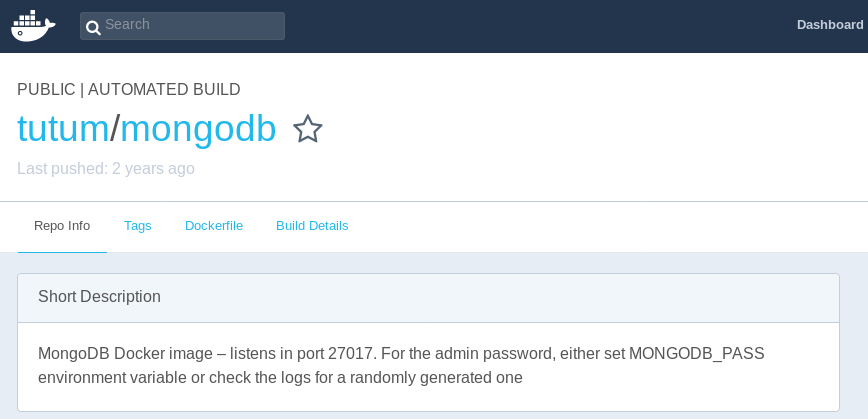
\includegraphics[width=15cm]{figuras/mongoNonOficial.png}}
\caption{Exemplo dun repositorio non oficial no Docker Hub.}
\label{mongoNonOficial}
\end{figure}

Na figura \ref{dockerOficial} pódese observar a aparición da frase ``\textit{Official repository}'', indicando que o repositorio en cuestión provén dunha fonte fiábel, mentres que na figura \ref{mongoNonOficial} pódese ver como se trata dun repositorio público, pero que non provén de fontes oficiais, senón dun usuario concreto.

\subsubsection{Medidas estendidas de seguridade}

O Docker Hub oferta medidas estendidas de seguridade para os repositorios de fontes oficiais, como son a identificación e clasificación de vulnerabilidades segundo o seu nivel de risco. Por exemplo, se consultamos a etiqueta (\textit{tag}) correspondente á derradeira versión considerada estábel do \gls{SXBD} MongoDB\footnote{\url{https://www.mongodb.com/}} (\textit{3.6.4-jessie} arestora), podemos observar como o Docker Hub indícanos a aparición dun total de 13 compoñentes vulnerábeis, entre os 102 que conforman a imaxe. Amais, estes compoñentes son analizados segundo a capa á que pertenzan e clasificados segundo o seu nivel de risco. Esta información pode ser consultada na figura \ref{mongoOficialVulnerabilidades}, e non se trata de información meramente cuantitativa, senón que tamén se indican explicitamente as vulnerabilidades atopadas e a fonte, tal e como pode ser observado na figura \ref{mongoOficialVulnerabilidades2}. Por exemplo, é posíbel observar como este repositorio posúe vulnerabilidades consideradas de nivel crítico asociadas á libraría {\it glibc 2.19-18+deb8u10}.\\

\begin{figure}
\centerline{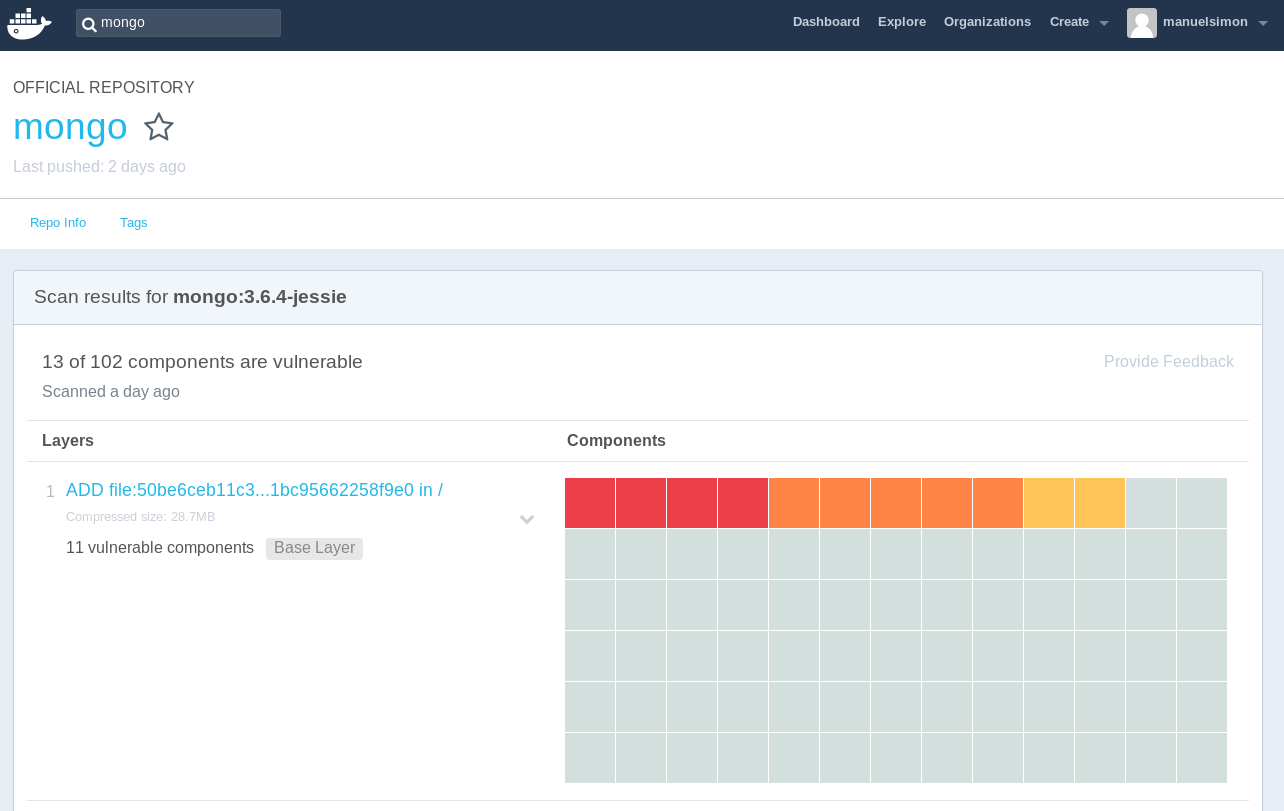
\includegraphics[width=15cm]{figuras/mongoOficialVulnerabilidades.png}}
\caption{Vulnerabilidades atopadas nun contedor oficial no Docker Hub. Parte 1.}
\label{mongoOficialVulnerabilidades}
\end{figure}

\begin{figure}
\centerline{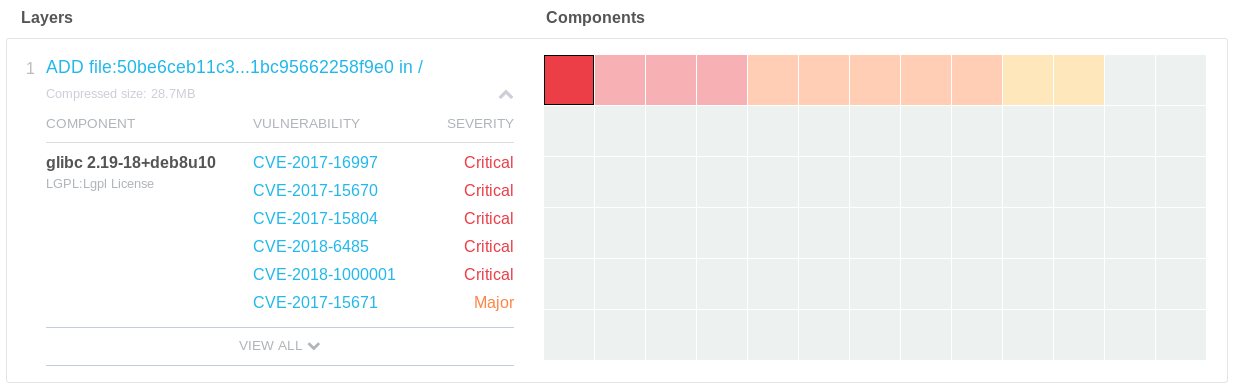
\includegraphics[width=15cm]{figuras/mongoOficialVulnerabilidades2.png}}
\caption{Vulnerabilidades atopadas nun contedor oficial no Docker Hub. Parte 2.}
\label{mongoOficialVulnerabilidades2}
\end{figure}

Este tipo de vulnerabilidades serán máis doadas de atopar canto máis complexa sexa a imaxe do contedor a montar, polo que é importante procurar seguir o principio da máxima simplicidade posíbel, empregando sempre un conxunto de contedores o máis simples que poidamos. Por exemplo, se consultamos no Docker Hub o repositorio dun \textit{Hello World}, podemos ver como non presenta ningún tipo de vulnerabilidade coñecida até o momento, tal e como ser apreciado nas figuras \ref{helloWorldSenVulnerabilidades} e \ref{helloWorldSenVulnerabilidades2}.

\begin{figure}
\centerline{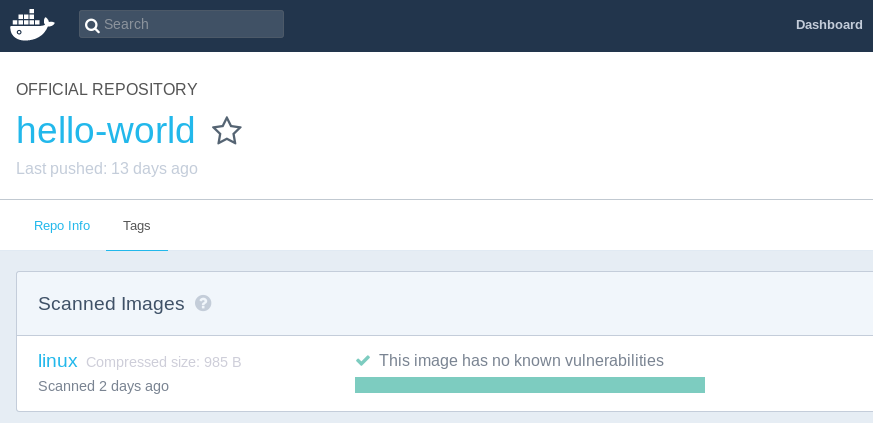
\includegraphics[width=15cm]{figuras/helloWorldSenVulnerabilidades.png}}
\caption{Repositorio \textit{Hello World} sen vulnerabilidades atopadas. Parte 1.}
\label{helloWorldSenVulnerabilidades}
\end{figure}

\begin{figure}
\centerline{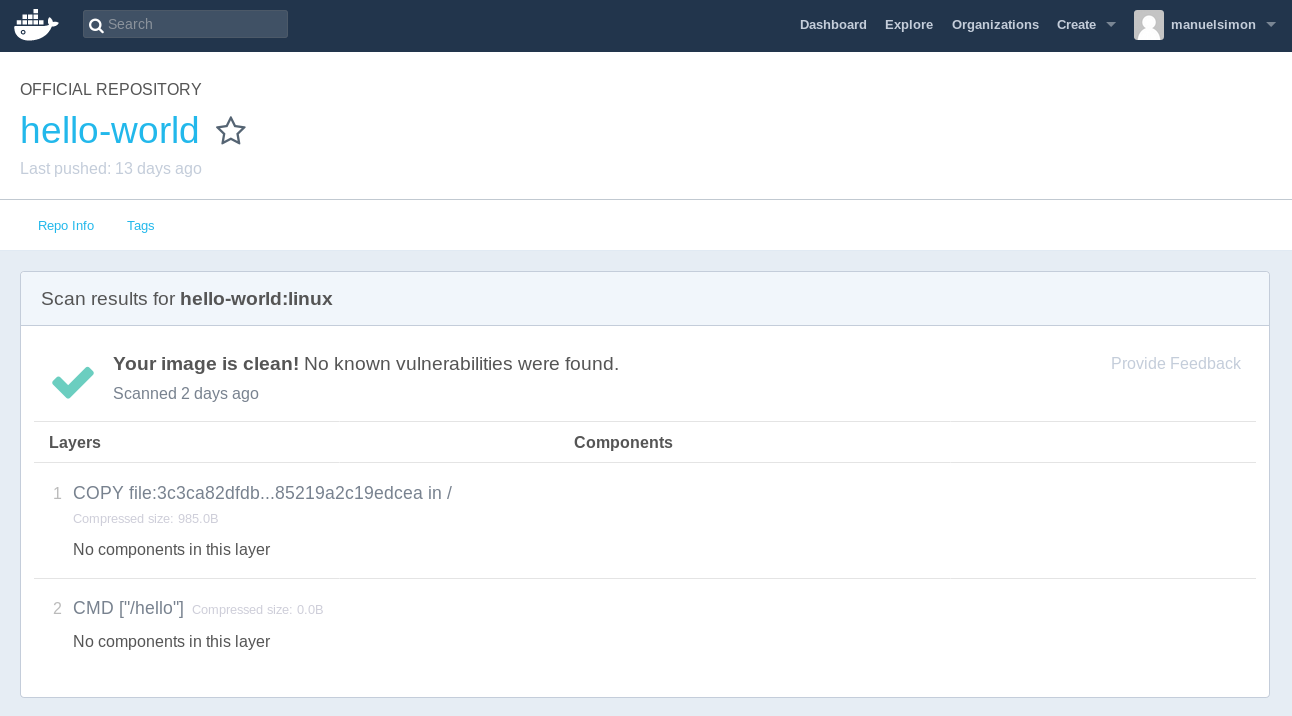
\includegraphics[width=15cm]{figuras/helloWorldSenVulnerabilidades2.png}}
\caption{Repositorio \textit{Hello World} sen vulnerabilidades atopadas. Parte 2.}
\label{helloWorldSenVulnerabilidades2}
\end{figure}

\subsubsection{Conclusións}

Polo tanto, endexamais debemos asumir que polo feito de estaren incluídos nun directorio centralizado, como pode ser o Docker Hub, os contedores están libres de vulnerabilidades. Deberiamos empregar contedores cuxas fontes, desenvolvedores ou repositorios sexan coñecidos e considerados de confianza, e na medida do posíbel, empregar soamente aqueles mantidos por unha fonte oficial ou comunidade.

\section{Herdanza de vulnerabilidades}

Continuando coa idea anteriormente presentada da posíbel dependencia entre imaxes mediante as relacións pai-fillo, dende o punto de vista da seguridade informática é importante remarcar que, aínda que esta é unha característica moi útil para reducir custos e engadir flexibilidade, coa dependencia entre imaxes tamén se probará calquera vulnerabilidade de software que a imaxe pai contivese se non son aplicadas as medidas e actualizacións de seguridade precisas \cite{studySecurityDockerHub}. Moitas veces, estas medidas pasan por simplemente actualizar as librarías no interior do contedor á súa última versión (por exemplo, aplicando un {\tt apt-get update \&\& apt-get upgrade}). A importancia de manter o sistema actualizado quedará representada na sección \ref{actualizacionSistema}. Asemade, evidenciando os riscos de seguridade que implican estas dependencias entre imaxes, Rui Shu, Xiaohui Gu e William Enck levaron a cabo un estudo (``\textit{A Study of Security Vulnerabilities on Docker Hub}'' \cite{studySecurityDockerHub}) no que realizaron múltiples análises e entre as cales podemos atopar un exemplo de herdanza de vulnerabilidades entre imaxes dependentes. Este exemplo pode ser contemplado na figura \ref{herdanzaVulnerabilidades}.

\begin{figure}
\centerline{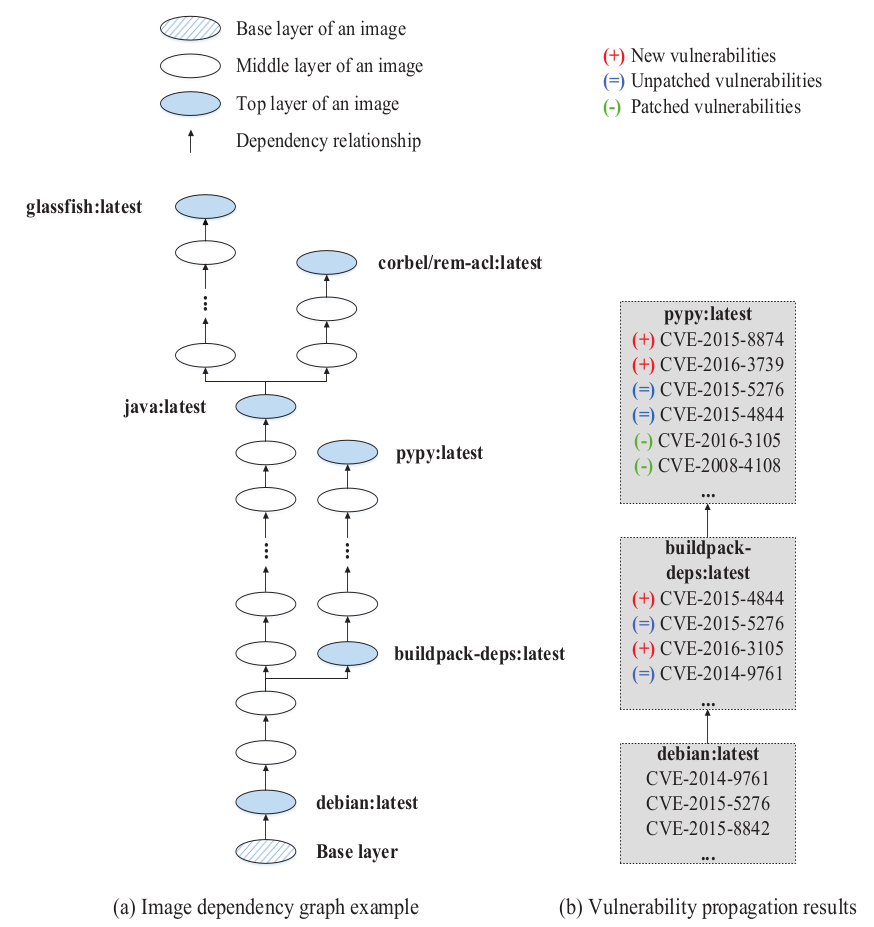
\includegraphics[width=15cm]{figuras/herdanzaVulnerabilidades.png}}
\caption{Exemplo de herdanza de vulnerabilidades}
\medskip
\small
\centerline{Fonte: \cite{studySecurityDockerHub}}
\label{herdanzaVulnerabilidades}
\end{figure}

\section{Detección de vulnerabilidades con Clair}

\subsection{Necesidade da ferramenta}

Os contedores poden incluír vulnerabilidades xa coñecidas no seu interior, tendo importantes implicacións de seguridade. Para evitar expor o noso sistema é importante ter coñecemento das posíbeis consecuencias que pode traer o despregamento de certo contedor. Aínda que algúns rexistros de imaxes, como pode ser o Docker Hub, xa inclúen mecanismos para informarnos acerca das vulnerabilidades atopadas en certas imaxes, non sempre faremos uso de fontes con mecanismos de seguridade tan avanzados, senón que é posíbel que cheguen contedores de múltiples fontes das que non será tan sinxelo obter unha información tan detallada. Ademais, tamén cabe a posibilidade de que tras facer cambios no contedor, tivésemos creado sen sabelo un entorno que inclúe vulnerabilidades. Debido a estes feitos, cómpre aplicar políticas propias de detección de vulnerabilidades en imaxes previo ao seu despregamento como contedores no entorno ou antes de proseguir cun proceso de integración continua.\\

Unha alternativa para realizar unha análise dos contedores pode tratarse do proxecto de código aberto Clair, o cal realiza unha análise estática de vulnerabilidades en contedores. Actualmente inclúe suporte para contedores Docker e appc \cite{clair}, pero existen adaptacións para a análise de contedores propios de Singularity.

\subsection{Funcionamento}

Esta ferramenta extraerá información tal como: 1) a versión dos paquetes de software instalados ou 2) os metadatos do sistema operativo en cada unha das capas que conforman a imaxe. A información detallada pode ser consultada na táboa \ref{datosClair}.\\

\begin{table}[]
\centering
\caption{Datos recollidos por Clair}
\label{datosClair}
\resizebox{\textwidth}{!}{%
\begin{tabular}{|c|c|}
\hline
\textbf{Nome do campo} & \textbf{Descrición}\\ \hline
\textit{Timestamp} & Data exacta do análise \\ \hline
ID da vulnerabilidade & Identificador unívoco da vulnerabilidade no \gls{CVE}\\ \hline
Nivel de gravidade & Clasificación da gravidade da vulnerabilidade\\ \hline
Descrición do \gls{CVE} & Descrición de cada vulnerabilidade identificada\\ \hline
Paquetes asociados & Nome e versión exacta dos paquetes vulnerábeis\\ \hline
Identificador da capa & Indicador da capa onde reside a vulnerabilidade atopada\\ \hline
\end{tabular}
}
\end{table}

Os datos sobre vulnerabilidades son importados continuamente dende un conxunto coñecido de fontes e son correlacionados cos contidos indexados das imaxes dos contedores para xerar listas de vulnerabilidades que poñen en risco aos mesmos \cite{clairWeb}. Clair identifica os paquetes inseguros realizando emparellamentos entre os metadatos e as listas de vulnerabilidades coñecidas (\gls{CVE}s). Cabe destacar que Clair soamente indentifica a presenza de paquetes con vulnerabilidades coñecidas; non determina se eses paquetes van ser empregados verdadeiramente, nin tampouco existe a posibilidade de detectar un comportamento dinámico nos contedores unha vez instanciados (por exemplo, novos paquetes vulnerábeis poderían ser instalados nos contedores en execución). \cite{studySecurityDockerHub} \\

Clair pode ser integrado directamente cun rexistro de contedores, automatizando o escaneo de imaxes e establecendo un mecanismo seguro para a notificación de vulnerabilidades, o que permitirá fornecer a seguridade do noso sistema. A arquitectura final desta ferramenta quedaría entón conformada por unhas fontes fiábeis de vulnerabilidades coñecidas, das que se obtería a información para ser gardada nunha base de datos relacional xestionada polo \gls{SXBD} PostgreSQL\footnote{\url{https://www.postgresql.org/}}, o nomeado rexistro de imaxes e, finalmente, un punto final de notificación das vulnerabilidades atopadas. Dita arquitectura está representada na figura \ref{clair-diagram}.

\begin{figure}
\centerline{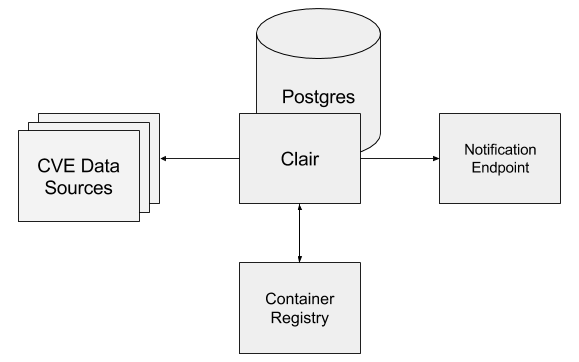
\includegraphics[width=15cm]{figuras/clair-diagram.png}}
\caption{Arquitectura de Clair}
\small
\centerline{Fonte: \url{https://github.com/coreos/clair/blob/master/Documentation/running-clair.md}}
\label{clair-diagram}
\end{figure}

\subsection{Probas}

Nesta sección serán realizadas unha serie de probas para amosar o funcionamento da ferramenta Clair, así como para deixar patentes os riscos asociados á emprega de imaxes sen ter coñecemento das vulnerabilidades existentes nas mesmas.

\subsubsection{Docker}
\label{clairScannerDocker}

Para o estudo con contedores Docker, empregarase a ferramenta {\it clair-scanner} \footnote{\url{https://github.com/arminc/clair-scanner}}, a cal permite unha análise das vulnerabilidades das imaxes gardadas na propia máquina local. É dicir, rediriximos o rexistro á propia máquina local, simplificando a arquitectura habitual de Clair amosada na figura \ref{clair-diagram}. Os motivos que impulsan esta simplificación vén dados por: 1) estase a traballar cunha proba de concepto, 2) Clair non está implantado actualmente no sistema do \gls{FT2} e 3) a súa implantación non ten sentido actualmente, ao non existir tampouco soporte para Docker. Esta ferramenta tamén presenta a posibilidade de comparar as vulnerabilidades atopadas cunha lista branca, na cal é posíbel indicar vulnerabilidades que pasaremos por alto se fose a nosa vontade, acadando de tal xeito un alto nivel de flexibilidade. Posto que estamos a substituír o rexistro por imaxes atopadas na propia máquina local, esta proba non suporá un método automatizado de análise de imaxes como o que Clair pode chegar a acadar. No entanto, xa que non existe actualmente un rexistro de contedores no \gls{CESGA}, a proba a realizar exemplificará perfectamente o funcionamento de Clair sen precisar deste compoñente.\\

O proceso de emprega de Clair pasaría polas seguintes fases:

\begin{enumerate}
    \item Un desenvolvedor de software obtén unha imaxe ou crea o seu contedor e envía unha imaxe do mesmo a Clair.
    \item Clair analiza a imaxe, na procura de vulnerabilidades de seguridade.
    \item Clair devolve un informe detallado das vulnerabilidades de seguridade atopadas na imaxe.
    \item O desenvolvedor actúa en base ao informe.
        \begin{itemize}
            \item Procura unha solución alternativa solucionando as vulnerabilidades.
            \item Con coñecemento da súa existencia, asume os riscos asociados ás vulnerabilidades e adiciona as mesmas á lista branca.
        \end{itemize}
\end{enumerate}

A análise mediante a nomeada ferramenta efectúase seguindo os seguintes comandos:

\begin{lstlisting}[,caption={Análise de imaxes de contedores mediante \textit{clair-scanner}}]
docker run -p 5432:5432 -d --name db arminc/clair-db:`date -d "-2 day" '+%Y-%m-%d'`
docker run -p 6060:6060 --link db:postgres -d --name clair arminc/clair-local-scan:v2.0.1
clair-scanner --ip 172.17.0.1 $IMAGEID
\end{lstlisting}

\begin{figure}
\centerline{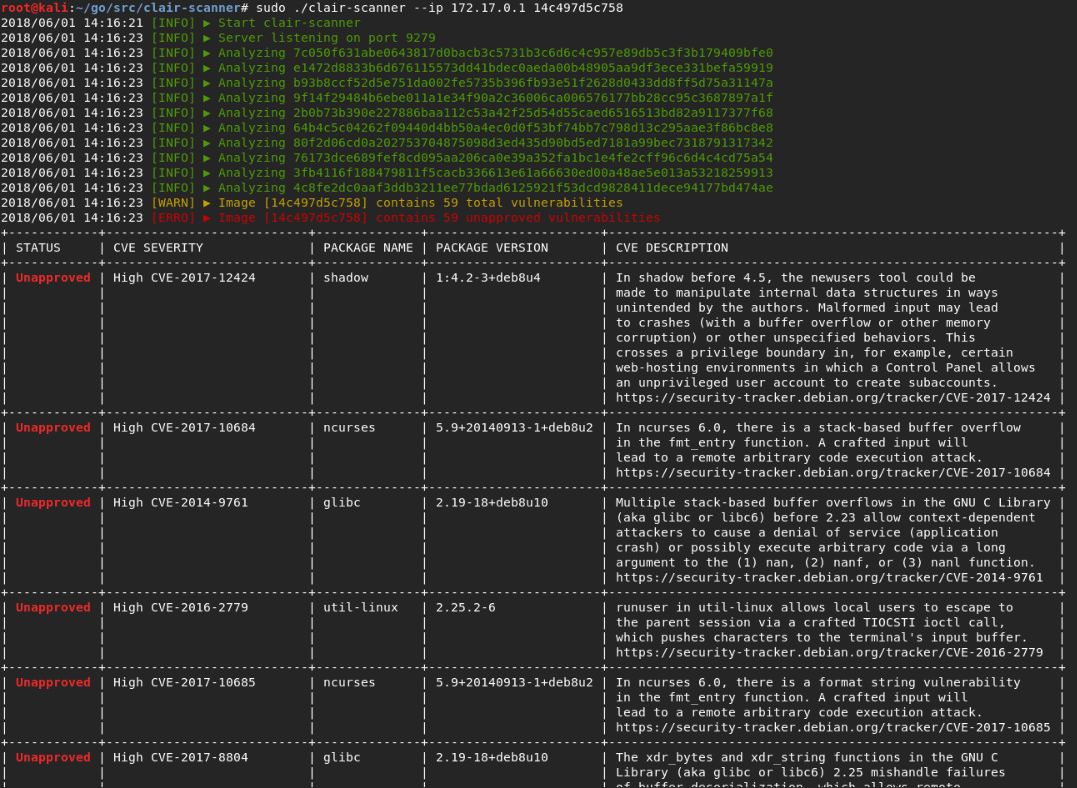
\includegraphics[width=15cm]{figuras/clairDocker.png}}
\caption{Exemplo de execución de {\it clair-scanner}}
\label{clairDocker}
\end{figure}

Isto equivalería a despregar un contedor coa base de datos de vulnerabilidades actualizada e outro contedor coa ferramenta Clair. Finalmente invocamos ao {\it clair-scanner} e amósanos os resultados das vulnerabilidades atopadas sobre a imaxe, tal e como pódese ver na figura \ref{clairDocker}.

\subsubsection{Singularity}

Existe unha adaptación de Clair para traballar sobre contedores Singularity\footnote{\url{https://github.com/dctrud/clair-singularity}}. O seu funcionamento baséase no feito de que un arquivo \textit{.tar.gz} exportado dunha imaxe Singularity é similar a unha imaxe dunha única capa dun contedor Docker. Polo tanto, esta ferramenta:

\begin{enumerate}
    \item Exporta unha imaxe Singularity a un arquivo temporal \textit{.tar.gz}.
    \item Calcula o \textit{hash} \gls{SHA}-256 como nome único a dar a Clair.
    \item Envía o arquivo \textit{.tar.gz} a través dun servidor \gls{HTTP} incorporado, mediante o cal Clair pode recuperalo.
    \item Chama á \gls{API} de Clair para que analice o arquivo \textit{.tar.gz} como unha capa para o análise.
    \item Chama á \gls{API} de Clair para o obter o informe de vulnerabilidades.
    \item Amosa os resultados por pantalla.
\end{enumerate}

Dita ferramenta aínda non posúe soporte para certificados de cliente \gls{SSL}, polo que non é posíbel verificar que estamos a enviar solicitudes a unha instancia Clair fiábel. Polo tanto, dita solución resulta insegura a non ser que a empreguemos baixo un entorno illado local. Este tipo de entorno foi o escollido para desenvolver as probas que se amosan a continuación.

\begin{lstlisting}[,caption={Análise dunha imaxe \textit{Hello-World} Singularity}]
bash-4.3# singularity build hello-world.simg docker://hello-world
Docker image path: index.docker.io/library/hello-world:latest
Cache folder set to /root/.singularity/docker
[1/1] |===================================| 100.0% 
Importing: base Singularity environment
Importing: /root/.singularity/docker/sha256:9bb5a5d4561a5511fa7f80718617e67cf2ed2e6cdcd02e31be111a8d0ac4d6b7.tar.gz
Importing: /root/.singularity/metadata/sha256:942999de4612d732c9e2b49bcd0633781edd5f3bd457d5f4f6cdc965b1abef9e.tar.gz
Building Singularity image...
Singularity container built: hello-world.simg
Cleaning up...

bash-4.3# sclair hello-world.simg 
Found 27 Clair namespaces
Clair URL: http://127.0.0.1:6060/v1

1. Starting server...
======== Running on http://127.0.0.1:8080 ========
(Press CTRL+C to quit)

1. Checking server...
2. Processing images!
Exporting hello-world.simg to targz...
2.4.5-dist
...exported hello-world.simg to /tmp/tmpo39pub_w/singularity-clair.d1hbbu74.tar.gz
...serving http://127.0.0.1:8080/images/singularity-clair.d1hbbu74.tar.gz to Clair
3. Generating report!
hello-world.simg does not have any vulnerabilities!
\end{lstlisting}

Como pode ser apreciado no código anterior, unha imaxe Docker é descargada dende o repositorio do Docker Hub e é adaptada a Singularity, grazas aos servizos de importación cos que conta esta tecnoloxía de contedorización. Posteriormente é analizada pola adaptación da ferramenta Clair para imaxes Singularity. Rematado o escáner, é posíbel apreciar como esta imaxe non presenta ningunha vulnerabilidade coñecida, tal e como xa puideramos ollar no repositorio do Docker Hub de onde provén, ao ser unha imaxe moi simple.\\

Seguindo o mesmo procedemento que no caso anterior, o Clair analizou nunha nova execución unha imaxe adaptada a Singularity correspondente ao Mongo DB, na súa versión \textit{3.6.4-jessie}. Como amosan os resultados, esta imaxe si que presenta vulnerabilidades coñecidas.

\begin{lstlisting}[,caption={Análise dunha imaxe MongoDB Singularity}]
bash-4.3# singularity build mongo.simg docker://mongo:3.6.4-jessie
Docker image path: index.docker.io/library/mongo:3.6.4-jessie
Cache folder set to /root/.singularity/docker
[10/10] |===================================| 100.0% 
Importing: base Singularity environment
Importing: /root/.singularity/docker/sha256:4d0d76e05f3c6caf923a71ca3b3d2cc8c834ca61779ae6b6d83547f3dd814980.tar.gz
.
.
.
Importing: /root/.singularity/metadata/sha256:2087064d2efc26145ab24e8a245e92d56e97c9e6df934621d02524aab46bea19.tar.gz
Building Singularity image...
Singularity container built: mongo.simg
Cleaning up...

bash-4.3# sclair mongo.simg 

Found 27 Clair namespaces
Clair URL: http://127.0.0.1:6060/v1

1. Starting server...
======== Running on http://127.0.0.1:8080 ========
(Press CTRL+C to quit)

1. Checking server...
2. Processing images!
Exporting mongo.simg to targz...
2.4.5-dist
...exported mongo.simg to /tmp/tmpvds_0eom/singularity-clair.k964yxz7.tar.gz
...serving http://127.0.0.1:8080/images/singularity-clair.k964yxz7.tar.gz to Clair
3. Generating report!
gnupg - 1.4.18-7+deb8u4
-----------------------
CVE-2018-6829 (Negligible)
https://security-tracker.debian.org/tracker/CVE-2018-6829
cipher/elgamal.c in Libgcrypt through 1.8.2, when used to encrypt messages directly, improperly encodes plaintexts, which allows attackers to obtain sensitive information by reading ciphertext data (i.e., it does not have semantic security in face of a ciphertext-only attack). The Decisional Diffie-Hellman (DDH) assumption does not hold for Libgcrypt's ElGamal implementation.


shadow - 1:4.2-3+deb8u4
-----------------------
CVE-2017-12424 (High)
https://security-tracker.debian.org/tracker/CVE-2017-12424
In shadow before 4.5, the newusers tool could be made to manipulate internal data structures in ways unintended by the authors. Malformed input may lead to crashes (with a buffer overflow or other memory corruption) or other unspecified behaviors. This crosses a privilege boundary in, for example, certain web-hosting environments in which a Control Panel allows an unprivileged user account to create subaccounts.


CVE-2018-7169 (Medium)
https://security-tracker.debian.org/tracker/CVE-2018-7169
An issue was discovered in shadow 4.5. newgidmap (in shadow-utils) is setuid and allows an unprivileged user to be placed in a user namespace where setgroups(2) is permitted. This allows an attacker to remove themselves from a supplementary group, which may allow access to certain filesystem paths if the administrator has used "group blacklisting" (e.g., chmod g-rwx) to restrict access to paths. This flaw effectively reverts a security feature in the kernel (in particular, the /proc/self/setgroups knob) to prevent this sort of privilege escalation.


CVE-2007-5686 (Negligible)
https://security-tracker.debian.org/tracker/CVE-2007-5686
initscripts in rPath Linux 1 sets insecure permissions for the /var/log/btmp file, which allows local users to obtain sensitive information regarding authentication attempts.  NOTE: because sshd detects the insecure permissions and does not log certain events, this also prevents sshd from logging failed authentication attempts by remote attackers.
.
.
.
\end{lstlisting}

\subsubsection{Udocker}

Udocker emprega as mesmas imaxes de contedores que Docker, sendo completamente compatíbel con moitos dos aspectos desta tecnoloxía. Así, o estudo realizado coa ferramenta \textit{clair-scanner} na sección \ref{clairScannerDocker} sobre as imaxes de Docker é exportábel a esta tecnoloxía de contedorización.

\section{Conclusións}

Como foi visto ao longo deste capítulo, as imaxes que darán lugar aos contedores que conformarán parte do noso sistema non están en ningún momento libres de conter vulnerabilidades, algunhas pudendo chegar a ser consideradas críticas. O feito de que ditas imaxes estean almacenadas en repositorios como o Docker Hub, ou que incluso sexan cedidas polos seus propios desenvolvedores non impide que conteñan ditas vulnerabilidades.\\

Tamén foi vista a importancia de contar con unha ferramenta de análise de vulnerabilidades a nivel local e non depender de servizos externos, posto que a orixe das imaxes pode chegar a ser moi heteroxéneo.\\

Polo tanto, podemos concluír que cando tratamos con contedores, os riscos de seguridade xa veñen dados incluso antes de chegar a facer algo na nosa propia infraestrutura, ao empregar materiais de terceiros e incorporar numerosas librarías e dependencias novas no noso sistema. É importante contar cun sistema que permita coñecer as vulnerabilidades ás que estaremos expostos, de traballar con certas imaxes, de forma que poidamos solucionalas ou ben asumir os seus riscos, pero sempre dende o coñecemento da súa existencia.
